\documentclass[9pt,twocolumn,twoside]{pnas-new}
% Use the lineno option to display guide line numbers if required.

% ---------------------------------------------------------------------------
% HOW THIS FILE WORKS
%  * Every number in the text is a macro (e.g. \NumSongs) defined in results.tex,
%    which make_paper_assets.py writes from the data. Re-run the script after the
%    Genius download and recompile: all numbers, tables and figures update.
%  * Text in \Verify{...} (orange) is an interpretation that depends on what the real
%    data shows. Read each one against the numbers, edit it, then remove \Verify.
%    Search for "Verify" before handing in.
% ---------------------------------------------------------------------------
\usepackage{xcolor}
\usepackage{array}  % ragged-right table columns
% Let two full-width figures share the top of a page (avoids a page with a single figure)
\setcounter{dbltopnumber}{2}
\renewcommand{\dbltopfraction}{0.9}
\renewcommand{\dblfloatpagefraction}{0.8}
\usepackage{jabbrv} % journal abbreviations used by pnas-new.bst (already loaded by newer classes)
\newcommand{\Verify}[1]{{\color{orange}#1}}
% AUTO-GENERATED by make_paper_assets.py -- do not edit by hand
\newcommand{\WikiArtists}{322}
\newcommand{\WikiLinks}{2,282}
\newcommand{\WikiTopThree}{Britney Spears (68), Madonna (68), Beyonce (61)}
\newcommand{\WikiModularity}{0.25}
\newcommand{\DataStatus}{}
\newcommand{\YearMin}{2000}
\newcommand{\YearMax}{2025}
\newcommand{\SongsPerArtist}{30}
\newcommand{\LyricsPerArtist}{15}
\newcommand{\MinEdgeWeight}{2}
\newcommand{\NumArtists}{266}
\newcommand{\NumSongs}{5,081}
\newcommand{\NumSongsCredits}{4,951}
\newcommand{\NumGeniusMatched}{309}
\newcommand{\NumManualMatched}{39}
\newcommand{\NumNoSongs}{43}
\newcommand{\PctSongsCredits}{97}
\newcommand{\NumCreators}{5,694}
\newcommand{\NumBipEdges}{9,312}
\newcommand{\NumEdges}{2,578}
\newcommand{\Density}{0.073}
\newcommand{\AvgDegree}{19.4}
\newcommand{\GiantSize}{181}
\newcommand{\GiantPct}{68}
\newcommand{\NumIsolated}{85}
\newcommand{\Clust}{0.56}
\newcommand{\ClustER}{0.16}
\newcommand{\ClustConfig}{0.32}
\newcommand{\TopCreator}{Max Martin}
\newcommand{\TopCreatorArtists}{31}
\newcommand{\MedianCreatorArtists}{1}
\newcommand{\PctOneArtistCreators}{75}
\newcommand{\NumTopOnePct}{57}
\newcommand{\PctReachedTopOne}{53}
\newcommand{\BridgeArtist}{Gwen Stefani}
\newcommand{\Modularity}{0.20}
\newcommand{\ModNullMean}{0.14}
\newcommand{\ModNullStd}{0.01}
\newcommand{\NumComms}{6}
\newcommand{\NumCommsBig}{5}
\newcommand{\YearAssort}{0.19}
\newcommand{\NumSongsLyrics}{2,732}
\newcommand{\NumTokens}{225,409}
\newcommand{\KruskalH}{32.0}
\newcommand{\KruskalP}{p<0.001}
\newcommand{\HappyMean}{5.95}
\newcommand{\HappiestComm}{C2}
\newcommand{\HappiestVal}{6.03}
\newcommand{\SaddestComm}{C3}
\newcommand{\SaddestVal}{5.88}
\newcommand{\YearRho}{-0.08}
\newcommand{\YearRhoP}{p<0.001}
\newcommand{\SimLinked}{0.178}
\newcommand{\SimUnlinked}{0.138}
\newcommand{\SimRatio}{1.29}
\newcommand{\PermObserved}{0.178}
\newcommand{\PermNull}{0.145}
\newcommand{\PermP}{p<0.001}
\newcommand{\NumPerm}{1,000}
\newcommand{\WeightRho}{0.17}
\newcommand{\WeightRhoP}{p<0.001}
\newcommand{\SimSameComm}{0.152}
\newcommand{\SimDiffComm}{0.143}
\newcommand{\WikiNMI}{0.21}
\newcommand{\WikiNMINull}{0.10}
\newcommand{\PctCreditEdgesOnWiki}{26}
\newcommand{\PctRandomOnWiki}{8.2}
\newcommand{\ThetaOneGiant}{224}
\newcommand{\ThetaOneQ}{0.18}
\newcommand{\ThetaOneQNull}{0.10}
\newcommand{\ThetaOneSimObs}{0.168}
\newcommand{\ThetaOneSimNull}{0.132}
\newcommand{\ThetaOneP}{p<0.001}
\newcommand{\ThetaThreeGiant}{161}
\newcommand{\ThetaThreeQ}{0.24}
\newcommand{\ThetaThreeQNull}{0.19}
\newcommand{\ThetaThreeSimObs}{0.183}
\newcommand{\ThetaThreeSimNull}{0.152}
\newcommand{\ThetaThreeP}{p<0.001}

% Fallbacks so the file also compiles with older copies of pnas-new.cls (no effect on Overleaf):
\providecommand{\articletype}[1]{}
\providecommand{\Firstpage}{}
\providecommand{\Endparasplit}{}
\providecommand{\dataavail}[1]{\paragraph*{Data Availability.} #1}
\providecommand{\bibsplit}[1][]{}

\articletype{SOCIAL SCIENCES}%%%% Article topic/classification

\templatetype{pnasresearcharticle} % Choose template

\begin{document}

\title{A few hands behind the hits: songwriter networks and shared lyrics in contemporary pop music}

% TODO: add group members here if you work in a group.
\author[a,1]{Haukur Meth\'usalem \'Oskarsson}

\affil[a]{DTU Compute, Technical University of Denmark, 2800 Kongens Lyngby, Denmark}

\leadauthor{\'Oskarsson}

\significancestatement{Pop stars are the faces of pop music, but many of their hits are written by the same small group of professional songwriters and producers. We map these hidden connections by linking every artist to the people credited on their songs, which turns the pop industry into a network. We then ask whether the network leaves a trace in the music itself: do artists who share songwriters also use the same words and sound equally happy or sad? Combining network science with text analysis shows how a handful of creators can shape what millions of listeners hear.}

\authorcontributions{H.M.\'O. designed the study, collected the data, performed the analysis and wrote the paper.}
\authordeclaration{The author declares no competing interest.}
\correspondingauthor{\textsuperscript{1}To whom correspondence should be addressed. E-mail: TODO@student.dtu.dk}

\keywords{Songwriter networks $|$ Bipartite networks $|$ Community detection $|$ Text analysis $|$ Popular music}

\begin{abstract}
\DataStatus{} Popular music is credited to its singers, yet most hits are written by teams of professional songwriters and producers. We study this hidden structure using the credits of \NumSongs{} songs (\YearMin--\YearMax) by \NumArtists{} pop artists from Genius, together with the Wikipedia pages of \WikiArtists{} artists. We build a bipartite network of artists and the \NumCreators{} creators credited on their songs, and project it onto an artist network in which two artists are linked when they share at least \MinEdgeWeight{} songwriters or producers. Creator degrees are highly skewed: \PctOneArtistCreators\% of creators work with a single artist, while the top 1\% of creators, led by \TopCreator, together reach \PctReachedTopOne\% of all artists. Louvain community detection splits the artist network into communities with modularity $Q=\Modularity$ (degree-preserving null: $\ModNullMean \pm \ModNullStd$), which differ in era and in their characteristic vocabularies. Using TF-IDF and the LabMT happiness lexicon on \NumSongsLyrics{} English lyrics, we find that communities differ in emotional tone, although the differences are small (Kruskal--Wallis $H=\KruskalH$, $\KruskalP$). Finally, artists who share creators have lyrics that are more similar (mean cosine similarity \SimLinked{} vs.\ \SimUnlinked{} for unlinked pairs), and a permutation test shows that this is unlikely to be due to chance ($\PermP$). Together, these results suggest that a small set of songwriters and producers connects much of pop music and leaves a weak but measurable fingerprint in its words.
\end{abstract}

\dates{This manuscript was compiled on \today}
\doi{02805 Social Graphs and Interactions, Final Project}

\maketitle
\thispagestyle{firststyle}
\ifthenelse{\boolean{shortarticle}}{\ifthenelse{\boolean{singlecolumn}}{\abscontentformatted}{\abscontent}}{}

\Firstpage

\dropcap{W}hen we think of a pop song, we think of the singer. Yet the credits of most chart hits list several other names: songwriters who wrote the melody and lyrics, and producers who shaped the sound. Journalistic accounts describe a ``song machine'' in which a small number of professional hitmakers write for many of the biggest stars \cite{seabrook2015}. If this is true, pop music is not a set of independent artists but a densely connected system, held together by people the audience rarely sees.

Network science offers natural tools to study such a system. Collaboration networks of creative workers have been studied for Broadway musicals, where the structure of the team network was linked to commercial and artistic success \cite{uzzi2005}, and for jazz musicians, where communities reflected both geography and race \cite{gleiser2003}. Credits link two types of entities, artists and creators, so they form a bipartite network that can be projected onto either side \cite{newman2001random,zhou2007}. Text analysis offers a second lens. Lyrics carry topics and emotions, and large-scale studies of song content have shown that successful songs differ from the rest in measurable ways \cite{interiano2018}. Word-level happiness scores such as LabMT make it possible to measure the emotional tone of large text collections \cite{dodds2011}.

Here we combine both lenses. We ask four questions:
\begin{enumerate}
\item Is pop music held together by a small number of hub songwriters and producers?
\item Does the artist network split into communities, and do these match eras or styles?
\item Does each community have its own vocabulary and emotional tone?
\item Do artists who share songwriters also use more similar words?
\end{enumerate}
The last question links the two halves: if creators have a personal style, then the network of shared credits should predict lyrical similarity.\Endparasplit
% \Endparasplit ends the narrow first-page column. If the first page looks odd on
% Overleaf, move \Endparasplit to the end of the paragraph where the page breaks.

\section*{Results}

\subsection*{Data overview}
We collected \WikiArtists{} pop artists from Wikipedia (Materials and Methods) and matched \NumGeniusMatched{} of them to Genius, where we downloaded the \SongsPerArtist{} most popular songs per artist released between \YearMin{} and \YearMax{}. Of the matched artists, \NumNoSongs{} (mostly acts from the 1980s and 1990s) had no songs in this period. The final data set contains \NumSongs{} songs by \NumArtists{} artists; \PctSongsCredits\% of the songs list at least one songwriter or producer, and \NumSongsLyrics{} songs have usable English lyrics (\NumTokens{} tokens after cleaning). The bipartite artist--creator network has \NumCreators{} creators and \NumBipEdges{} edges. Projected onto artists, with an edge whenever two artists share at least \MinEdgeWeight{} creators, it has \NumEdges{} edges (average degree \AvgDegree, density \Density). Its giant component contains \GiantSize{} artists (\GiantPct\%); all network results below are for the giant component.

\subsection*{A few creators connect most of pop}
The number of artists per creator is extremely uneven (Fig.~\ref{fig:degrees}). Three in four creators (\PctOneArtistCreators\%) appear on songs by only one artist, whereas the most connected creator, \TopCreator, is credited on songs by \TopCreatorArtists{} different artists. The \NumTopOnePct{} best-connected creators (the top 1\%) together reach \PctReachedTopOne\% of all artists in the data. The list is dominated by the Scandinavian-American hit factory around \TopCreator{} (Stargate, Shellback, Savan Kotecha) and by producers such as Greg Kurstin, Dr.\ Luke and Cirkut (Table~\ref{tab:creators}). The top three by reach are also the top three by betweenness centrality, meaning that they sit on many of the shortest paths between otherwise separate parts of the network. Among artists, \BridgeArtist{} has the highest betweenness and acts as the main bridge between communities.

The projected artist network is strongly clustered (average clustering \Clust), far above Erd\H{o}s--R\'enyi graphs with the same density (\ClustER) and configuration-model graphs with the same degree sequence (\ClustConfig). Part of this is expected, since every creator turns the artists they worked with into a clique in the projection; the comparison mainly shows that credits come in tight, repeated teams rather than random pairings.

\begin{figure}[t]
\centering
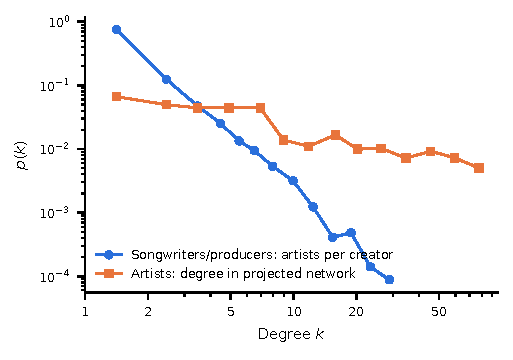
\includegraphics[width=\linewidth]{figures/fig2_degrees.pdf}
\caption{Degree distributions on log--log axes (logarithmic bins). Blue: number of distinct artists per songwriter/producer in the bipartite network. Orange: degree of artists in the projected artist network. The heavy tail for creators means that a few songwriters and producers work with a large share of all artists.}
\label{fig:degrees}
\end{figure}

\begin{table}[t]
\centering
\caption{The ten songwriters/producers credited on songs by the most artists. ``Songs'' counts credited songs in the data; ``Betw.'' is the rank by betweenness centrality in the bipartite network (1 = highest).}
\label{tab:creators}
\begin{tabular}{rlrrr}
\# & Songwriter/producer & Artists & Songs & Betw. \\
\midrule
1 & Max Martin & 31 & 114 & 3 \\
2 & Greg Kurstin & 26 & 82 & 1 \\
3 & Stargate & 26 & 57 & 2 \\
4 & Dr. Luke & 22 & 76 & 5 \\
5 & Cirkut & 22 & 70 & 10 \\
6 & Savan Kotecha & 21 & 45 & 8 \\
7 & Jacob Kasher & 21 & 49 & 11 \\
8 & benny blanco & 20 & 76 & 24 \\
9 & Ryan Tedder & 19 & 28 & 21 \\
10 & Justin Tranter & 19 & 43 & 36 \\
\bottomrule
\end{tabular}

\end{table}

\subsection*{Pop splits into families}
The Louvain method finds \NumComms{} communities in the giant component, \NumCommsBig{} of which have at least five artists (Fig.~\ref{fig:network}, Table~\ref{tab:communities}). The partition has modularity $Q=\Modularity$. This is modest in absolute terms, as the many edges between communities in Fig.~\ref{fig:network} show, but it is well above the $\ModNullMean \pm \ModNullStd$ obtained on degree-preserving randomizations of the network, so the communities are not an artifact of the degree sequence. They are recognisable families: a 2010s pop group around Katy Perry and Camila Cabello (C1), a 2000s group of largely British and European pop acts, girl groups and boy bands around Kelly Clarkson, Kylie Minogue and the Saturdays (C2), an R\&B and hip-hop group around Usher, Beyonc\'e and Rihanna (C3), a club and dance group around David Guetta, Flo Rida and Jennifer Lopez (C4), and a mainstream pop group around Britney Spears, Gwen Stefani and Kesha (C5). The communities are partly separated by time (median years from 2009 in C2 to 2017 in C1; Table~\ref{tab:communities}), and the median release year of an artist's songs is weakly assortative across edges ($r=\YearAssort$), so artists tend to share creators with artists from the same era, but genre separates the families more clearly than time.

As an independent check we compared the credit-based communities with communities in the network of hyperlinks between the artists' Wikipedia pages (\WikiLinks{} links; most linked-to pages: \WikiTopThree). The two partitions agree with normalized mutual information $\mathrm{NMI}=\WikiNMI$, compared with $\WikiNMINull$ for shuffled labels, and \PctCreditEdgesOnWiki\% of artist pairs that share creators also link to each other on Wikipedia, compared with \PctRandomOnWiki\% of all pairs. Shared credits therefore capture relations that Wikipedia editors also recognize, but the agreement is far from complete: most pairs of artists who share creators do not link to each other on Wikipedia.

\begin{figure*}[t]
\centering
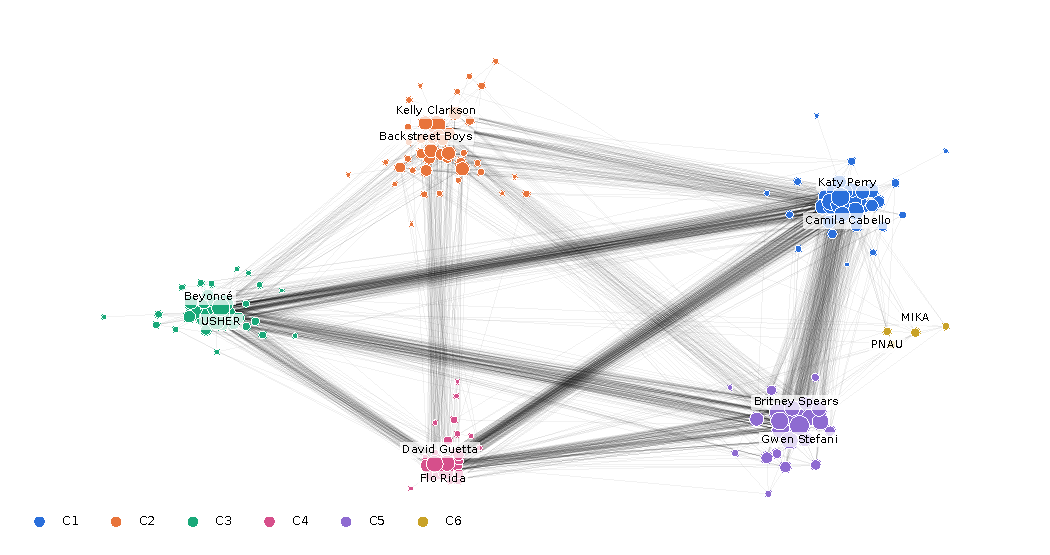
\includegraphics[width=\textwidth]{figures/fig1_network.pdf}
\caption{The pop artist network (giant component). Each node is an artist; two artists are linked if they share at least \MinEdgeWeight{} songwriters or producers. Node size grows with degree; colours mark the \NumComms{} Louvain communities (C1--C6). For readability each community is laid out separately and the communities are placed around a circle, so distances between communities carry no meaning; grey lines are edges. Labels show the two best-connected artists in each community. An interactive version is available on the project website.}
\label{fig:network}
\end{figure*}

\begin{table*}[t]
\centering
\caption{The Louvain communities of the artist network. ``Year'' is the median of the artists' median release years. Example artists are the three with the highest weighted degree. Top words are the community's highest-scoring terms (TF-IDF over artists, Materials and Methods). Happiness is the mean LabMT score per song ($\Delta h=1$).}
\label{tab:communities}
\begin{tabular*}{\textwidth}{@{\extracolsep{\fill}}lrr>{\raggedright\arraybackslash}p{4.6cm}>{\raggedright\arraybackslash}p{4.6cm}r@{}}
Comm. & Artists & Year & Best-connected artists & Top TF-IDF words & Happiness \\
\midrule
C1 & 42 & 2017 & Camila Cabello, Selena Gomez, Rita Ora & replaced, highs, hopeless, vulnerable, perfume & 5.93 \\
C2 & 42 & 2009 & Kelly Clarkson, The Saturdays, Jessica Simpson & pleasure, speaking, longing, neon, swept & 6.03 \\
C3 & 39 & 2011 & USHER, Beyonce, Rihanna & n*ggas, n*gga, denim, frontin, hoes & 5.88 \\
C4 & 30 & 2013 & Flo Rida, David Guetta, Jennifer Lopez & hooked, dale, criminal, miami, trigger & 6.00 \\
C5 & 24 & 2012 & Britney Spears, Gwen Stefani, Jessie J & odds, mrs, cruel, ideas, tattooed & 5.88 \\
C6 & 4 & 2015 & MIKA, PNAU, Empire of the Sun & meets, cannonball, gentle, setting, valley & 5.96 \\
\bottomrule
\end{tabular*}

\end{table*}

\begin{figure*}[t]
\centering
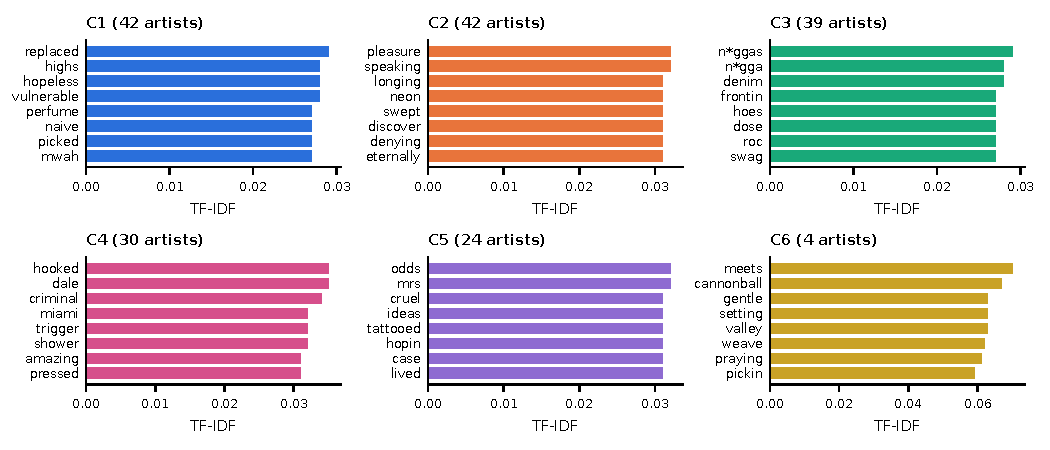
\includegraphics[width=\textwidth]{figures/fig3_words.pdf}
\caption{Characteristic words of the communities: the eight terms with the highest TF-IDF score, where term frequency is the number of artists in the community who use a word and inverse document frequency is taken over all artists (Materials and Methods). Colours match Fig.~\ref{fig:network}. Slurs are partly masked.}
\label{fig:words}
\end{figure*}

\begin{figure*}[t]
\centering
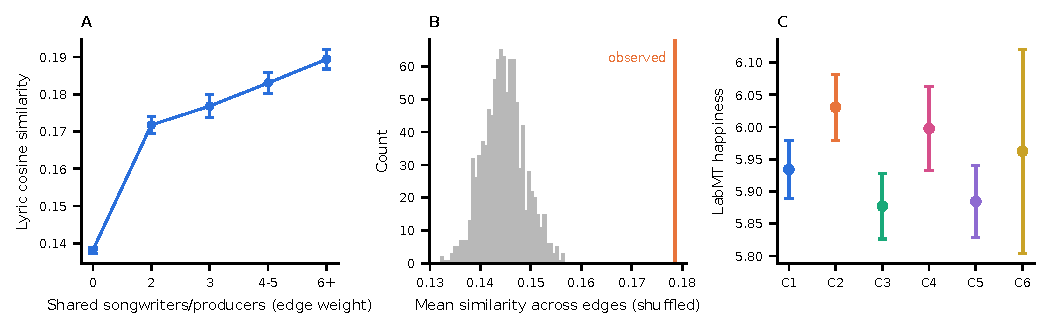
\includegraphics[width=\textwidth]{figures/fig4_similarity.pdf}
\caption{Network and lyrics. (\textit{A}) Mean lyric cosine similarity between pairs of artists as a function of the number of songwriters/producers they share (0 = not linked); error bars are 95\% confidence intervals. (\textit{B}) Mean similarity across the edges of the network when artists are randomly reassigned to nodes (grey, \NumPerm{} permutations) and in the real network (orange line). (\textit{C}) Mean LabMT happiness per song in each community with 95\% confidence intervals.}
\label{fig:similarity}
\end{figure*}

\subsection*{Each family has its own words and mood}
A TF-IDF score picks out words that many artists in a community use but few artists use overall (Fig.~\ref{fig:words}). The words match the genres of the families. The R\&B and hip-hop community C3 is marked by rap vocabulary (``frontin'', ``swag'', slurs and slang), the club community C4 by party and Latin words (``dale'', ``miami'', ``hooked'', ``criminal''), and the 2010s pop community C1 by an introspective, confessional vocabulary (``hopeless'', ``vulnerable'', ``naive'', ``replaced''). The 2000s community C2 sings about ``pleasure'', ``longing'' and ``eternally''. Most words are, however, shared across all communities: the top terms are characteristic, not exclusive.

Communities also differ in emotional tone. The mean LabMT happiness of a song is \HappyMean{} overall, ranging from \SaddestVal{} in \SaddestComm{} to \HappiestVal{} in \HappiestComm{} (Fig.~\ref{fig:similarity}C). The differences between communities are statistically significant (Kruskal--Wallis $H=\KruskalH$, $\KruskalP$) but small, about 0.15 on a scale from 1 to 9. Across all songs, happiness is correlated with release year with Spearman $\rho=\YearRho$ ($\YearRhoP$), so pop lyrics have become very slightly sadder over the period.

\subsection*{Shared songwriters, shared words}
Finally, we tested whether the credit network predicts what the lyrics say. Each artist was represented by a TF-IDF vector of all their lyrics, and we computed the cosine similarity between every pair of artists. Linked artists have a mean similarity of \SimLinked, compared with \SimUnlinked{} for unlinked pairs, a ratio of \SimRatio. Similarity rises steadily with the number of shared creators (Fig.~\ref{fig:similarity}A; Spearman $\rho=\WeightRho$, $\WeightRhoP$ among linked pairs), with the largest step between unlinked pairs and pairs that share two creators. Pairs in the same community are only slightly more similar than pairs in different communities (\SimSameComm{} vs.\ \SimDiffComm), so the effect is carried by direct links more than by community membership.

To test whether this could arise by chance, we kept the network fixed and randomly reassigned artists to nodes \NumPerm{} times. The mean similarity across edges was \PermObserved{} in the real network and \PermNull{} on average in the shuffled networks; no shuffled network came close ($\PermP$; Fig.~\ref{fig:similarity}B). Artists who share songwriters therefore use more similar words than expected by chance, although the absolute similarities are low and the difference is modest.

\section*{Discussion}
We set out to test whether pop music is held together by a small group of hidden creators, and whether this structure is visible in the lyrics. On the network side, the answer is largely yes: creator degrees are heavily skewed, the top 1\% of songwriters and producers reach about half of all artists, and the artist network splits into communities that are more modular than chance and correspond to recognisable genres and eras. The communities are, however, densely interconnected, so pop looks less like separate families than like one industry with a few overlapping neighbourhoods. On the text side, communities have characteristic vocabularies, and artists who share creators write more similar lyrics than expected under a permutation null. All text effects are small: happiness differs by less than 0.2 between communities, and linked artists are about 30\% more similar than unlinked ones.

This last result has an important caveat. Similar lyrics between linked artists could mean that creators bring a personal style to every artist they work with, but it could also mean that artists from the same era and genre both hire the same creators and sing about the same things. The vocabularies in Fig.~\ref{fig:words} support this concern, as they mostly reflect genre. Our permutation test rules out chance, but not this shared-context explanation. A stronger test would compare linked and unlinked pairs within the same community and the same release window, or regress similarity on shared credits while controlling for year and genre. We see this as the most important next step.

The data also have limits. Credits on Genius are crowd-sourced and incomplete, especially for older songs and smaller artists, so the network is a lower bound on the true collaboration structure. We use only the most popular songs of each artist, which favours hits and their (more professional) teams. Lyrics were analysed with a bag-of-words model and an English happiness lexicon, which ignores word order and irony, and we excluded non-English songs. Finally, Louvain communities vary slightly between runs and depend on the edge threshold $\theta$. We fixed the random seed and repeated the main tests for $\theta=1$ and $\theta=3$. The conclusions do not change: modularity is $\ThetaOneQ$ vs.\ $\ThetaOneQNull$ for the null at $\theta=1$ (giant component of \ThetaOneGiant{} artists) and $\ThetaThreeQ$ vs.\ $\ThetaThreeQNull$ at $\theta=3$ (\ThetaThreeGiant{} artists), and the mean lyric similarity across edges is \ThetaOneSimObs{} vs.\ \ThetaOneSimNull{} ($\ThetaOneP$) and \ThetaThreeSimObs{} vs.\ \ThetaThreeSimNull{} ($\ThetaThreeP$).

Despite these limits, the combination of credits and lyrics gives a simple, reproducible picture of how pop is made: a small core of professional creators who work across the whole industry, a few overlapping families of artists around them, and lyrics that carry a faint trace of who wrote them.

\matmethods{
\subsection*{Artist list (Wikipedia)}
We used the MediaWiki API to collect all article links on the Wikipedia page ``List of dance-pop artists'' and added a seed list of 45 widely known contemporary pop artists. Pages were downloaded in batches of 50 titles, and we kept only pages with an \texttt{Infobox musical artist} (or an \texttt{Infobox person} describing a singer, musician, songwriter or rapper), which removes links to genres, magazines and record labels. This gave \WikiArtists{} artists. Hyperlinks between these pages define a directed network with \WikiLinks{} edges, used for validation.

\subsection*{Songs, credits and lyrics (Genius)}
Each artist was matched to Genius by searching for the page title (without disambiguation such as ``(singer)'') and accepting a hit only if the normalized names agreed exactly. Unmatched artists were checked by hand, and \NumManualMatched{} were matched manually (e.g.\ ``Pink (singer)'' to P!nk, ``Teddy Sinclair'' to Natalia Kills); the remaining unmatched pages were mostly producers, a music critic and acts without a Genius page. For each artist we requested the \SongsPerArtist{} most popular songs on which they are the primary artist, and kept songs released between \YearMin{} and \YearMax. For every song we stored the credited writers, producers and featured artists. Genius credits the production duo Stargate sometimes as a team and sometimes as its two members; we merged these into one creator. Lyrics were downloaded for the \LyricsPerArtist{} most popular songs per artist with the \texttt{lyricsgenius} package. All API responses were cached, and lyrics are not redistributed.

\subsection*{Networks}
Let $w_{ac}$ be the number of songs by artist $a$ on which creator $c$ is credited as writer or producer (an artist's own credit on their own songs is ignored). The bipartite network has an edge $(a,c)$ with weight $w_{ac}$ whenever $w_{ac}>0$. The projected artist network has weights
\begin{equation}
W_{ab} = \left|\,\mathcal{N}(a) \cap \mathcal{N}(b)\,\right|,
\end{equation}
the number of creators shared by artists $a$ and $b$, and we keep an edge if $W_{ab}\geq\theta$ with $\theta=\MinEdgeWeight$, which removes many weak links created by single prolific creators.

\subsection*{Network measures}
We report degree distributions with logarithmic bins, the average clustering coefficient, and compare with 10 Erd\H{o}s--R\'enyi graphs \cite{erdos1959} with the same number of nodes and density and 10 configuration-model graphs \cite{molloy1995} with the same degree sequence. Betweenness centrality \cite{brandes2001} was estimated from 500 sampled source nodes. Communities were found with the Louvain method \cite{blondel2008}, which maximizes the weighted modularity \cite{newman2006}
\begin{equation}
Q = \frac{1}{2m}\sum_{ij}\left[W_{ij} - \frac{s_i s_j}{2m}\right]\delta(c_i, c_j),
\end{equation}
where $s_i$ is the strength of node $i$ and $m$ the total edge weight. As a null model we ran Louvain on 20 randomized networks obtained by degree-preserving double-edge swaps. Assortativity by median release year was measured with Newman's coefficient \cite{newman2003}. Credit-based and Wikipedia-based communities were compared with normalized mutual information, with a null obtained by shuffling community labels 200 times.

\subsection*{Text analysis}
Lyrics were cleaned by removing section headers (e.g.\ ``[Chorus]''), keeping each distinct line once (so repeated choruses do not dominate), lower-casing and tokenizing into alphabetic words. Because the stop words and the happiness lexicon are English, we kept only songs in which at least 25\% of the words are English stop words (English lyrics typically have about 45\%), which removes songs in Swedish, Spanish, French, Korean and other languages. We removed English stop words, contractions such as ``I'm'' and ``don't'', and a short list of filler words common in lyrics (``oh'', ``yeah'', ``baby'', \ldots). For each artist $g$ we computed TF-IDF weights \cite{salton1988}
\begin{equation}
\mathrm{tfidf}(t,g) = \left(1+\ln f_{t,g}\right)\left(\ln\frac{1+N}{1+n_t}+1\right),
\end{equation}
where $f_{t,g}$ is the count of term $t$ in the lyrics of $g$, $N$ the number of artists and $n_t$ the number of artists using $t$; vectors were $L_2$-normalized. For the characteristic words of a community $g$ we used the same formula with $f_{t,g}$ replaced by the number of artists in the community who use $t$, and kept words of at least three letters used by at least five artists. With only a handful of communities, an inverse document frequency over communities is nearly flat (most words occur in all of them), and raw counts let a single song that repeats a word define a whole community; counting artists avoids both problems. Emotional tone was measured with the LabMT lexicon \cite{dodds2011}: the happiness of a text is
\begin{equation}
h(T) = \frac{\sum_i h_i f_i}{\sum_i f_i}, \quad \text{over words with } |h_i - 5| \geq \Delta h,
\end{equation}
with $h_i$ the LabMT score of word $i$, $f_i$ its frequency and $\Delta h = 1$ to ignore neutral words. Differences between communities were tested with a Kruskal--Wallis test and trends over time with Spearman correlation.

\subsection*{Linking network and text}
Lyric similarity between artists $a$ and $b$ is the cosine similarity $s_{ab}=\mathbf{v}_a\cdot\mathbf{v}_b/(\|\mathbf{v}_a\|\|\mathbf{v}_b\|)$ of their TF-IDF vectors (one document per artist, terms in at least two artists). The test statistic is the mean similarity across edges, $\bar{s}=\frac{1}{|E|}\sum_{(a,b)\in E}s_{ab}$. Under the null hypothesis that lyrics are unrelated to network position, we randomly permuted which artist occupies which node $R=1{,}000$ times and computed $p=(1+\#\{\bar{s}^{(r)}\geq\bar{s}\})/(1+R)$.

\subsection*{Software}
All analysis used Python with NetworkX \cite{hagberg2008}, scikit-learn, pandas and SciPy. The full pipeline, from download to every number and figure in this paper, is in the accompanying repository.
}

\showmatmethods{} % Display the Materials and Methods section

\dataavail{Code is available at \Verify{TODO: GitHub link}. Wikipedia text is available under CC BY-SA. Song metadata were obtained from the Genius API; lyrics are copyrighted and are not redistributed, but can be re-downloaded with the provided code.}

\acknow{This work was carried out as the final project of the course 02805 Social Graphs and Interactions at the Technical University of Denmark.}

\showacknow{} % Display the acknowledgments section

\bibsplit[3]
% Use \bibsplit to split the references from the body of the text. Value "[3]" represents the number of reference in the left column.

\bibliography{references}

\end{document}
